\documentclass[tikz,border=0pt]{standalone}
% Shared flat Beamer-blue style; widths include padding.
\usepackage[T1]{fontenc}
\usepackage{lmodern}
\usepackage{tikz}
\usetikzlibrary{arrows.meta}
\definecolor{beamerblue}{RGB}{51,51,178}
\tikzset{
block/.style={rectangle,draw=beamerblue,fill=beamerblue!9,line width=.6pt,
minimum height=17mm,minimum width=34mm,text width=30mm,inner xsep=2mm,
inner ysep=1mm,align=center,text=black,font=\sffamily\fontsize{8}{9.5}\selectfont},
architecture/.style={block,minimum width=27mm,text width=23mm},
flow/.style={-{Stealth[length=1.6mm,width=1.2mm]},draw=beamerblue!65,line width=.75pt},
edge label/.style={font=\sffamily\fontsize{6}{7}\selectfont,text=black,align=center,inner sep=0pt}}
\newcommand{\heading}[1]{{\bfseries\fontsize{8.5}{10}\selectfont #1}}

\begin{document}
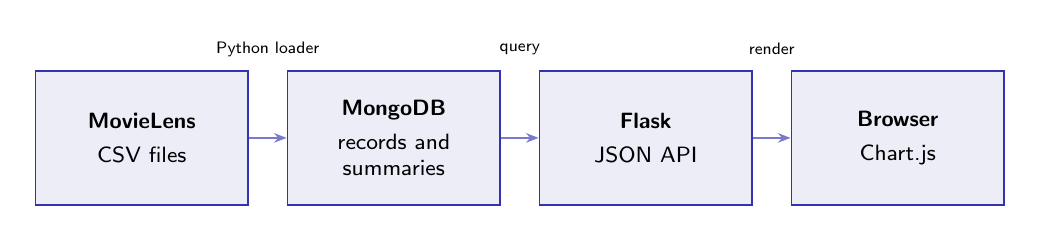
\begin{tikzpicture}[x=1mm,y=1mm]
  \path[use as bounding box,fill=white] (-14.5,-9.5) rectangle (110.5,14);
  \node[architecture] (n0) at (0,0) {\heading{MovieLens}\\[1mm]CSV files};
  \node[architecture] (n1) at (32,0) {\heading{MongoDB}\\[1mm]records and\\summaries};
  \node[architecture] (n2) at (64,0) {\heading{Flask}\\[1mm]JSON API};
  \node[architecture] (n3) at (96,0) {\heading{Browser}\\[1mm]Chart.js};
  \draw[flow] (n0.east) -- (n1.west);
  \draw[flow] (n1.east) -- (n2.west);
  \draw[flow] (n2.east) -- (n3.west);
  \node[edge label] at (16,11.3) {Python loader};
  \node[edge label] at (48,11.3) {query};
  \node[edge label] at (80,11.3) {render};
\end{tikzpicture}
\end{document}
